\documentclass{standalone}
\usepackage{tikz}
\usetikzlibrary{patterns, positioning}

\begin{document}
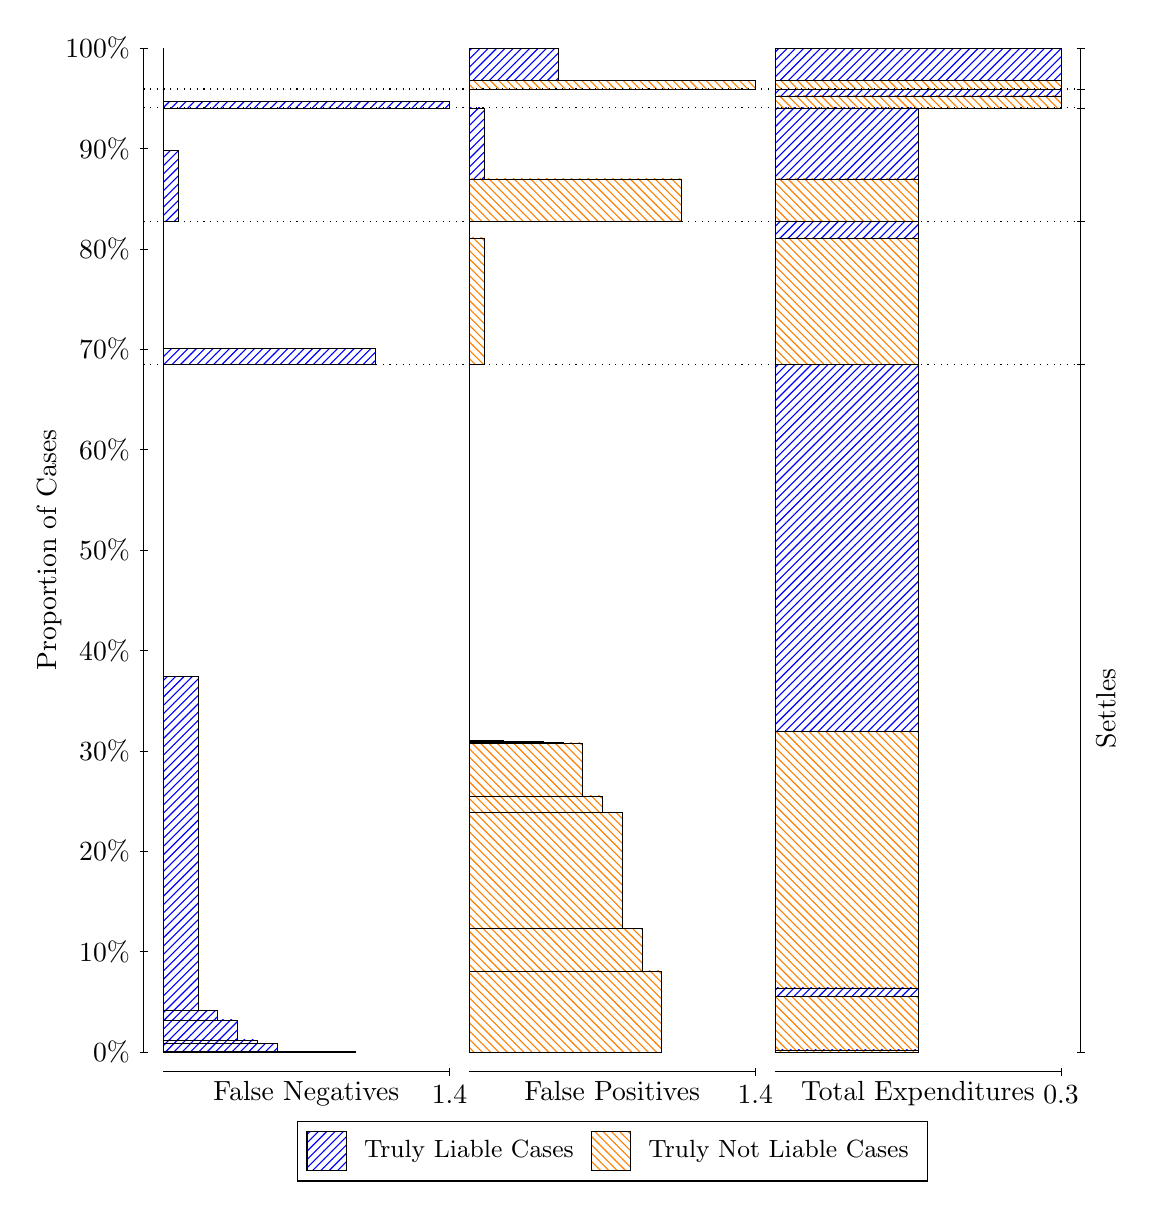
\begin{tikzpicture}
\draw[black, very thin] (1.5,1.75) -- (1.5,14.5);
\node[rotate=90, anchor=center] at (0.3, 8.125) {Proportion of Cases};
\draw[black, very thin] (1.45,1.75) -- (1.55,1.75);
\node[anchor=east] at (1.45, 1.75) {0\%};
\draw[black, very thin] (1.45,3.025) -- (1.55,3.025);
\node[anchor=east] at (1.45, 3.025) {10\%};
\draw[black, very thin] (1.45,4.3) -- (1.55,4.3);
\node[anchor=east] at (1.45, 4.3) {20\%};
\draw[black, very thin] (1.45,5.575) -- (1.55,5.575);
\node[anchor=east] at (1.45, 5.575) {30\%};
\draw[black, very thin] (1.45,6.85) -- (1.55,6.85);
\node[anchor=east] at (1.45, 6.85) {40\%};
\draw[black, very thin] (1.45,8.125) -- (1.55,8.125);
\node[anchor=east] at (1.45, 8.125) {50\%};
\draw[black, very thin] (1.45,9.4) -- (1.55,9.4);
\node[anchor=east] at (1.45, 9.4) {60\%};
\draw[black, very thin] (1.45,10.675) -- (1.55,10.675);
\node[anchor=east] at (1.45, 10.675) {70\%};
\draw[black, very thin] (1.45,11.95) -- (1.55,11.95);
\node[anchor=east] at (1.45, 11.95) {80\%};
\draw[black, very thin] (1.45,13.225) -- (1.55,13.225);
\node[anchor=east] at (1.45, 13.225) {90\%};
\draw[black, very thin] (1.45,14.5) -- (1.55,14.5);
\node[anchor=east] at (1.45, 14.5) {100\%};

\draw[black, very thin] (13.4,1.75) -- (13.4,14.5);
\draw[black, very thin] (13.35,1.75) -- (13.45,1.75);
\node[anchor=west] at (13.35, 1.75) {};
\draw[black, very thin] (13.35,10.479) -- (13.45,10.479);
\node[anchor=west] at (13.35, 10.479) {};
\draw[black, very thin] (13.35,12.294) -- (13.45,12.294);
\node[anchor=west] at (13.35, 12.294) {};
\draw[black, very thin] (13.35,13.741) -- (13.45,13.741);
\node[anchor=west] at (13.35, 13.741) {};
\draw[black, very thin] (13.35,13.979) -- (13.45,13.979);
\node[anchor=west] at (13.35, 13.979) {};
\draw[black, very thin] (13.35,14.5) -- (13.45,14.5);
\node[anchor=west] at (13.35, 14.5) {};

\draw[black, very thin, pattern color=blue, pattern=north east lines] (1.75,1.75) rectangle (4.1931,1.7537);
\draw[black, very thin, pattern color=blue, pattern=north east lines] (1.75,1.7537) rectangle (3.9425,1.7542);
\draw[black, very thin, pattern color=blue, pattern=north east lines] (1.75,1.7542) rectangle (3.692,1.758);
\draw[black, very thin, pattern color=blue, pattern=north east lines] (1.75,1.758) rectangle (3.4414,1.7623);
\draw[black, very thin, pattern color=blue, pattern=north east lines] (1.75,1.7623) rectangle (3.1908,1.8628);
\draw[black, very thin, pattern color=blue, pattern=north east lines] (1.75,1.8628) rectangle (2.9402,1.9031);
\draw[black, very thin, pattern color=blue, pattern=north east lines] (1.75,1.9031) rectangle (2.6897,2.1584);
\draw[black, very thin, pattern color=blue, pattern=north east lines] (1.75,2.1584) rectangle (2.4391,2.2779);
\draw[black, very thin, pattern color=blue, pattern=north east lines] (1.75,2.2779) rectangle (2.1885,6.5235);
\draw[black, very thin, pattern color=orange, pattern=north west lines] (1.75,6.5235) rectangle (1.75,10.479);
\draw[black, very thin, pattern color=blue, pattern=north east lines] (1.75,10.479) rectangle (4.4437,10.683);
\draw[black, very thin, pattern color=orange, pattern=north west lines] (1.75,10.683) rectangle (1.75,12.294);
\draw[black, very thin, pattern color=blue, pattern=north east lines] (1.75,12.294) rectangle (1.9379,13.198);
\draw[black, very thin, pattern color=orange, pattern=north west lines] (1.75,13.198) rectangle (1.75,13.741);
\draw[black, very thin, pattern color=blue, pattern=north east lines] (1.75,13.741) rectangle (5.3833,13.827);
\draw[black, very thin, pattern color=orange, pattern=north west lines] (1.75,13.827) rectangle (1.75,13.979);
\draw[black, very thin, pattern color=orange, pattern=north west lines] (1.75,13.979) rectangle (1.75,14.092);
\draw[black, very thin, pattern color=blue, pattern=north east lines] (1.75,14.092) rectangle (1.75,14.5);
\draw[black, very thin, pattern color=orange, pattern=north west lines] (5.6333,1.75) rectangle (8.0764,2.7792);
\draw[black, very thin, pattern color=orange, pattern=north west lines] (5.6333,2.7792) rectangle (7.8259,3.3189);
\draw[black, very thin, pattern color=orange, pattern=north west lines] (5.6333,3.3189) rectangle (7.5753,4.795);
\draw[black, very thin, pattern color=orange, pattern=north west lines] (5.6333,4.795) rectangle (7.3247,5.0037);
\draw[black, very thin, pattern color=orange, pattern=north west lines] (5.6333,5.0037) rectangle (7.0741,5.6763);
\draw[black, very thin, pattern color=orange, pattern=north west lines] (5.6333,5.6763) rectangle (6.8236,5.682);
\draw[black, very thin, pattern color=orange, pattern=north west lines] (5.6333,5.682) rectangle (6.8236,5.6844);
\draw[black, very thin, pattern color=orange, pattern=north west lines] (5.6333,5.6844) rectangle (6.573,5.6931);
\draw[black, very thin, pattern color=orange, pattern=north west lines] (5.6333,5.6931) rectangle (6.3224,5.6945);
\draw[black, very thin, pattern color=orange, pattern=north west lines] (5.6333,5.6945) rectangle (6.0718,5.7059);
\draw[black, very thin, pattern color=blue, pattern=north east lines] (5.6333,5.7059) rectangle (5.6333,10.479);
\draw[black, very thin, pattern color=orange, pattern=north west lines] (5.6333,10.479) rectangle (5.8213,12.09);
\draw[black, very thin, pattern color=blue, pattern=north east lines] (5.6333,12.09) rectangle (5.6333,12.294);
\draw[black, very thin, pattern color=orange, pattern=north west lines] (5.6333,12.294) rectangle (8.327,12.837);
\draw[black, very thin, pattern color=blue, pattern=north east lines] (5.6333,12.837) rectangle (5.8213,13.741);
\draw[black, very thin, pattern color=orange, pattern=north west lines] (5.6333,13.741) rectangle (5.6333,13.893);
\draw[black, very thin, pattern color=blue, pattern=north east lines] (5.6333,13.893) rectangle (5.6333,13.979);
\draw[black, very thin, pattern color=orange, pattern=north west lines] (5.6333,13.979) rectangle (9.2667,14.092);
\draw[black, very thin, pattern color=blue, pattern=north east lines] (5.6333,14.092) rectangle (6.7609,14.5);
\draw[black, very thin, pattern color=orange, pattern=north west lines] (9.5167,1.75) rectangle (11.333,1.7682);
\draw[black, very thin, pattern color=blue, pattern=north east lines] (9.5167,1.7682) rectangle (11.333,1.7768);
\draw[black, very thin, pattern color=orange, pattern=north west lines] (9.5167,1.7768) rectangle (11.333,2.4608);
\draw[black, very thin, pattern color=blue, pattern=north east lines] (9.5167,2.4608) rectangle (11.333,2.565);
\draw[black, very thin, pattern color=orange, pattern=north west lines] (9.5167,2.565) rectangle (11.333,5.8187);
\draw[black, very thin, pattern color=blue, pattern=north east lines] (9.5167,5.8187) rectangle (11.333,10.479);
\draw[black, very thin, pattern color=orange, pattern=north west lines] (9.5167,10.479) rectangle (11.333,12.09);
\draw[black, very thin, pattern color=blue, pattern=north east lines] (9.5167,12.09) rectangle (11.333,12.294);
\draw[black, very thin, pattern color=orange, pattern=north west lines] (9.5167,12.294) rectangle (11.333,12.837);
\draw[black, very thin, pattern color=blue, pattern=north east lines] (9.5167,12.837) rectangle (11.333,13.741);
\draw[black, very thin, pattern color=orange, pattern=north west lines] (9.5167,13.741) rectangle (13.15,13.893);
\draw[black, very thin, pattern color=blue, pattern=north east lines] (9.5167,13.893) rectangle (13.15,13.979);
\draw[black, very thin, pattern color=orange, pattern=north west lines] (9.5167,13.979) rectangle (13.15,14.092);
\draw[black, very thin, pattern color=blue, pattern=north east lines] (9.5167,14.092) rectangle (13.15,14.5);
\draw[black, dotted] (1.5,10.479) -- (13.4,10.479);
\draw[black, dotted] (1.5,12.294) -- (13.4,12.294);
\draw[black, dotted] (1.5,13.741) -- (13.4,13.741);
\draw[black, dotted] (1.5,13.979) -- (13.4,13.979);
\draw[black, very thin] (1.75,1.5) -- (5.3833,1.5);
\node[anchor=north] at (3.5667, 1.5) {False Negatives};
\draw[black, very thin] (5.3833,1.45) -- (5.3833,1.55);
\node[anchor=north] at (5.3833, 1.45) {1.4};

\draw[black, very thin] (5.6333,1.5) -- (9.2667,1.5);
\node[anchor=north] at (7.45, 1.5) {False Positives};
\draw[black, very thin] (9.2667,1.45) -- (9.2667,1.55);
\node[anchor=north] at (9.2667, 1.45) {1.4};

\draw[black, very thin] (9.5167,1.5) -- (13.15,1.5);
\node[anchor=north] at (11.333, 1.5) {Total Expenditures};
\draw[black, very thin] (13.15,1.45) -- (13.15,1.55);
\node[anchor=north] at (13.15, 1.45) {0.3};

\node[black, centered, rotate=90] at (13.72, 6.1147) {Settles};





\draw (7.449999999999999,1.5) node[draw=none] (baseCoordinate) {};
\begin{scope}[align=center]
        \matrix[scale=0.5, draw=black, below=0.5cm of baseCoordinate, nodes={draw}, column sep=0.1cm]{
            \node[rectangle, draw, minimum width=0.5cm, minimum height=0.5cm, pattern=north east lines, pattern color=blue] {}; &
            \node[draw=none, font=\small] (B) {Truly Liable Cases}; &
            \node[rectangle, draw, minimum width=0.5cm, minimum height=0.5cm, pattern=north west lines, pattern color=orange] {}; &
            \node[draw=none, font=\small] (B) {Truly Not Liable Cases}; \\
            };
\end{scope}

\end{tikzpicture}
\end{document}